\paragraph{QuizziPedia::Front-End::Controllers::InputToListController}
\begin{figure} [ht]
	\centering
	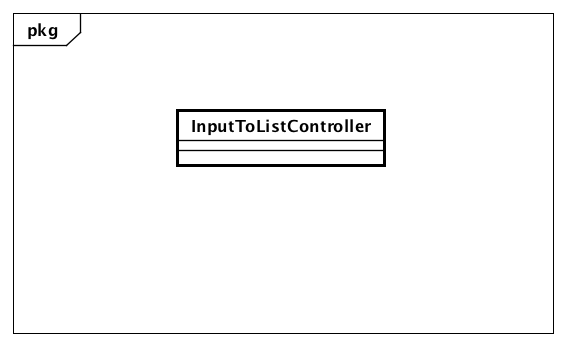
\includegraphics[scale=0.45]{UML/Classi/Front-End/QuizziPedia_Front-end_Controller_InputToListController.png}
	\caption{QuizziPedia::Front-End::Controllers::InputToListController}
\end{figure} \FloatBarrier
\begin{itemize}
	\item \textbf{Descrizione}: questa classe permette di gestire l'inserimento di una lista di risposte durante la creazione di una domanda;
	\item \textbf{Utilizzo}: fornisce le funzionalità per confermare porzioni di domanda durante la creazione;
	\item \textbf{Relazione con altre classi}:
	\begin{itemize}
		\item \textit{OUT} \texttt{MultipleQuestionsModelView}: classe di tipo modelview la cui istanziazione è contenuta all'interno della variabile di ambiente \$scope di \textit{Angular.js\ped{G}}. All'interno di essa sono presenti le variabili e i metodi necessari per il \textit{Two-Way Data-Binding\ped{G}} tra la view \texttt{MultipleQuestionsView} e il controller \texttt{MultipleQuestionsController};
		\item \textit{OUT} \texttt{ConnectionQuestionsModelView}: classe di tipo modelview la cui istanziazione è contenuta all'interno della variabile di ambiente \$scope di \textit{Angular.js\ped{G}}. All'interno di essa sono presenti le variabili e i metodi necessari per il \textit{Two-Way Data-Binding\ped{G}} tra la view \texttt{ConnectionQuestionView} e il controller \texttt{ConnectionQuestionController};
		\item \textit{OUT} \texttt{StringsSortingQuestionsModelView}: classe di tipo modelview la cui istanziazione è contenuta all'interno della variabile di ambiente \$scope di \textit{Angular.js\ped{G}}. All'interno di essa sono presenti le variabili e i metodi necessari per il \textit{Two-Way Data-Binding\ped{G}} tra la view \texttt{StringsSortingQuestionView} e il controller \texttt{StringsSortingQuestionController}; 
		\item \textit{OUT} \texttt{ImagesSortingQuestionsModelView}: permette all'utente di creare una domanda a ordinamento immagini compilando i campi proposticlasse di tipo modelview la cui istanziazione è contenuta all'interno della variabile di ambiente \$scope di \textit{Angular.js\ped{G}}. All'interno di essa sono presenti le variabili e i metodi necessari per il \textit{Two-Way Data-Binding\ped{G}} tra la view \texttt{ImagesSortingQuestionView} e il controller \texttt{ImagesSortingQuestionController};
	\end{itemize}
	\item \textbf{Attributi}:
	\begin{itemize}
		\item \texttt{-} \texttt{\$scope: \$scope} \\
		Campo dati contenente un riferimento all’oggetto \$scope creato da \textit{Angular\ped{G}}, viene utilizzato come mezzo di comunicazione tra il controller e la view. Contiene gli oggetti che definiscono il model dell’applicazione.
	\end{itemize}
	\item \textbf{Metodi}:
	\begin{itemize}
		\item \texttt{+} \texttt{InputToListController(\$scope: \$scope)} \\Metodo costruttore della classe. \\
		\textbf{Parametri}:
		\begin{itemize}
			\item \texttt{-} \texttt{\$scope: \$scope} \\
			Parametro contenente un riferimento all’oggetto \$scope creato da \textit{Angular\ped{G}}, viene utilizzato come mezzo di comunicazione tra il controller e la view. Contiene gli oggetti che definiscono il model dell’applicazione. 
		\end{itemize}
		\item \texttt{-} \texttt{putDownAnswer(): void} \\Metodo che reagisce all'evento di aggiunta nuova risposta e la salva in modo che venga caricata e visualizzata nella pagina.
	\end{itemize}
\end{itemize}

